\section{The Exploratory Campaigns}
\label{sec:exploratory}

Seven groups of campaigns ran on the same build with the same protocol (30
runs per cell, the same machine state, start delay and warm-up rules).
Three of them (the engine arms, the counters, the grain by threads) were
used in Section~\ref{sec:why}. The rest bound the primary results: they say
how far the two answers reach. All are exploratory: 95\% intervals, no
correction, no primary conclusion rests on them.

\subsection{Atomics without sharing, atomics with false sharing, sorts}
\label{sec:extras}

The extras campaign (5400 runs, 16.5 hours) measured a ladder at the two
ends of the contention sweep: local counters, \emph{private} atomics (one
padded table per thread), shared padded atomics, and \emph{packed} shared
atomics (eight counters per line), plus two parallel sorts
(Table~\ref{tab:extras}, Figures~\ref{fig:extras-speedup}
to~\ref{fig:extras-rq2}).

\begin{table}[htbp]
\caption{Extras campaign (5400 runs): time in ms at $N=1$ and 8, speedup at $N=8$ with its 95\,\% interval, and the time at $N=8$ over the native one.}\label{tab:extras}
\centering\scriptsize
\resizebox{\linewidth}{!}{%
\begin{tabular}{lrrcrrcrrrcr}
\toprule
 & \multicolumn{3}{c}{Native} & \multicolumn{4}{c}{Chrome} & \multicolumn{4}{c}{Firefox} \\
Workload & $T_1$ & $T_8$ & $S_8$ & $T_1$ & $T_8$ & $S_8$ & /nat. & $T_1$ & $T_8$ & $S_8$ & /nat. \\
\midrule
atomic, $k$=1 & 379.6 & 878.0 & 0.432 [0.421, 0.444] & 698.0 & 1805.4 & 0.387 [0.374, 0.400] & 2.06 & 379.7 & 891.5 & 0.426 [0.414, 0.439] & 1.02 \\
packed, $k$=1 & 381.2 & 878.8 & 0.434 [0.422, 0.446] & 699.9 & 1871.1 & 0.374 [0.360, 0.389] & 2.13 & 380.1 & 886.0 & 0.429 [0.418, 0.440] & 1.01 \\
private, $k$=1 & 379.6 & 47.674 & 7.963 [7.957, 7.968] & 697.9 & 88.031 & 7.928 [7.923, 7.933] & 1.85 & 379.7 & 47.800 & 7.944 [7.937, 7.950] & 1.00 \\
local, $k$=1 & 154.9 & 19.475 & 7.955 [7.952, 7.958] & 150.7 & 19.008 & 7.927 [7.917, 7.937] & 0.98 & 155.6 & 19.775 & 7.871 [7.861, 7.879] & 1.02 \\
\midrule
atomic, $k$=256 & 379.6 & 414.6 & 0.915 [0.914, 0.917] & 411.9 & 210.3 & 1.959 [1.958, 1.960] & 0.51 & 379.8 & 392.8 & 0.967 [0.966, 0.968] & 0.95 \\
packed, $k$=256 & 379.8 & 490.3 & 0.775 [0.772, 0.777] & 407.7 & 725.7 & 0.562 [0.560, 0.563] & 1.48 & 379.8 & 492.0 & 0.772 [0.769, 0.775] & 1.00 \\
private, $k$=256 & 379.6 & 47.677 & 7.961 [7.952, 7.970] & 411.6 & 52.110 & 7.900 [7.892, 7.907] & 1.09 & 379.9 & 47.835 & 7.941 [7.934, 7.948] & 1.00 \\
local, $k$=256 & 27.104 & 3.422 & 7.921 [7.898, 7.943] & 33.391 & 4.195 & 7.960 [7.861, 8.068] & 1.23 & 34.528 & 4.139 & 8.341 [8.189, 8.530] & 1.21 \\
\midrule
sort & 1468.0 & 188.5 & 7.789 [7.786, 7.793] & 1600.0 & 205.8 & 7.775 [7.773, 7.778] & 1.09 & 1531.7 & 196.3 & 7.802 [7.799, 7.804] & 1.04 \\
sort-unstable & 539.2 & 84.358 & 6.392 [6.389, 6.396] & 683.6 & 109.9 & 6.221 [6.217, 6.224] & 1.30 & 682.1 & 110.2 & 6.187 [6.182, 6.191] & 1.31 \\
\bottomrule
\end{tabular}
}
\end{table}


\begin{figure}[tbp]
\centering
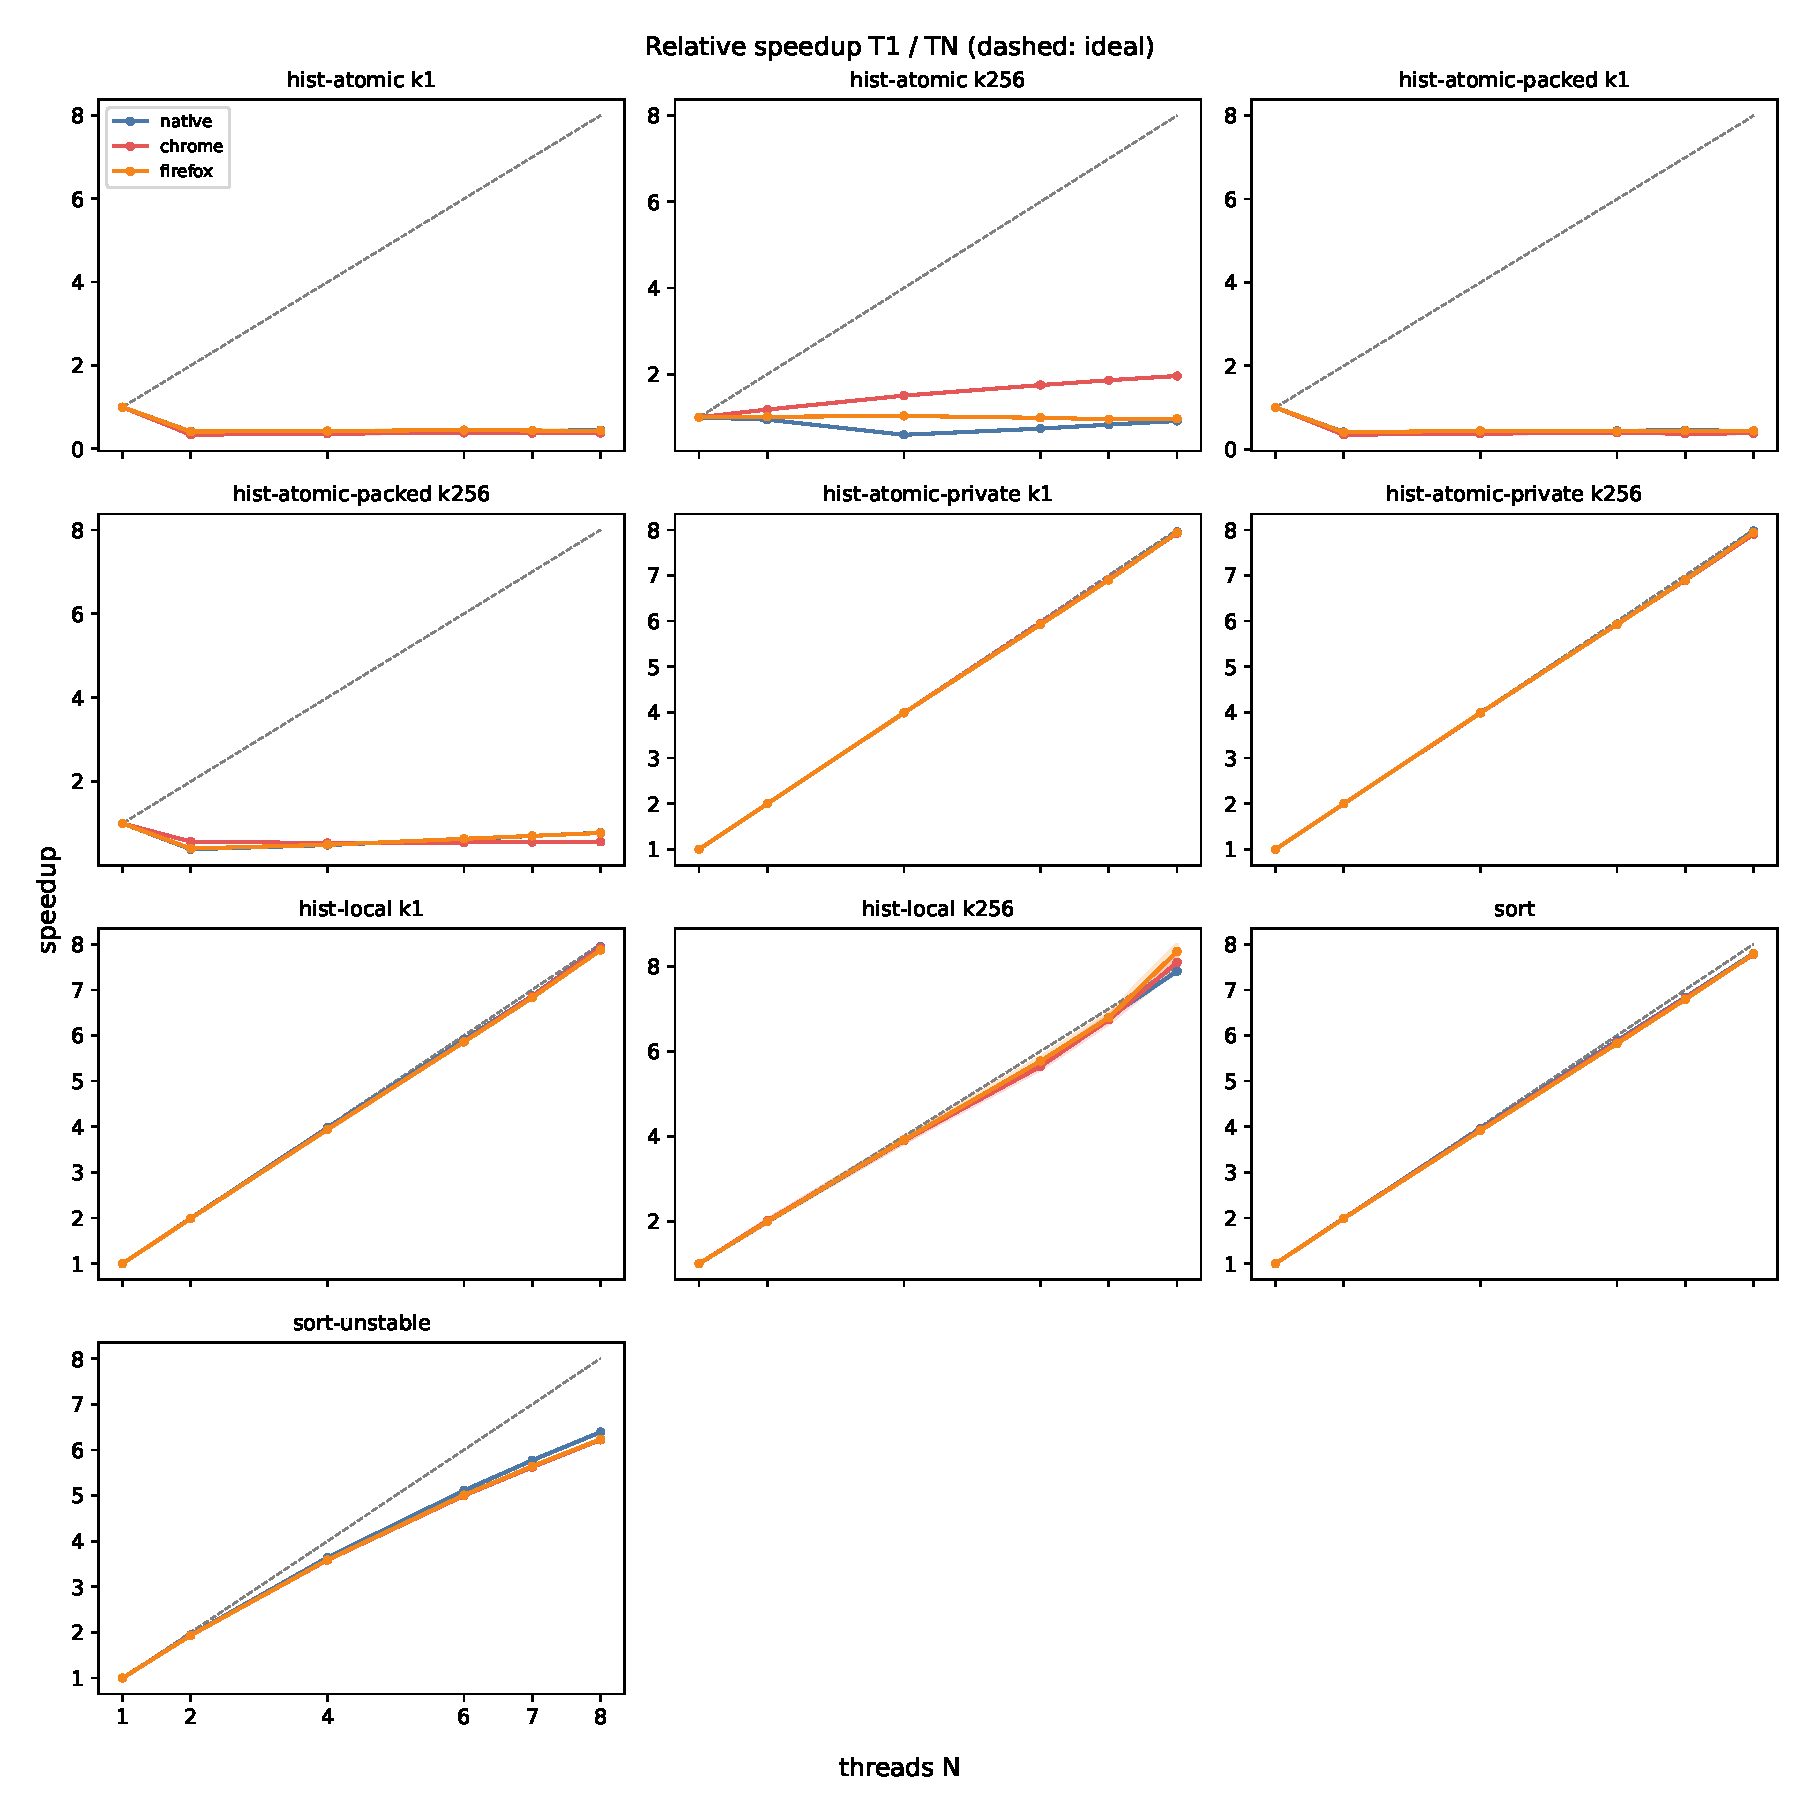
\includegraphics[width=0.8\linewidth]{../figures/extras-speedup.pdf}
\caption{Extras campaign: relative speedup per workload.}
\Description{Speedup against thread count for the extras workloads in the three environments.}
\label{fig:extras-speedup}
\end{figure}

\begin{figure}[tbp]
\centering
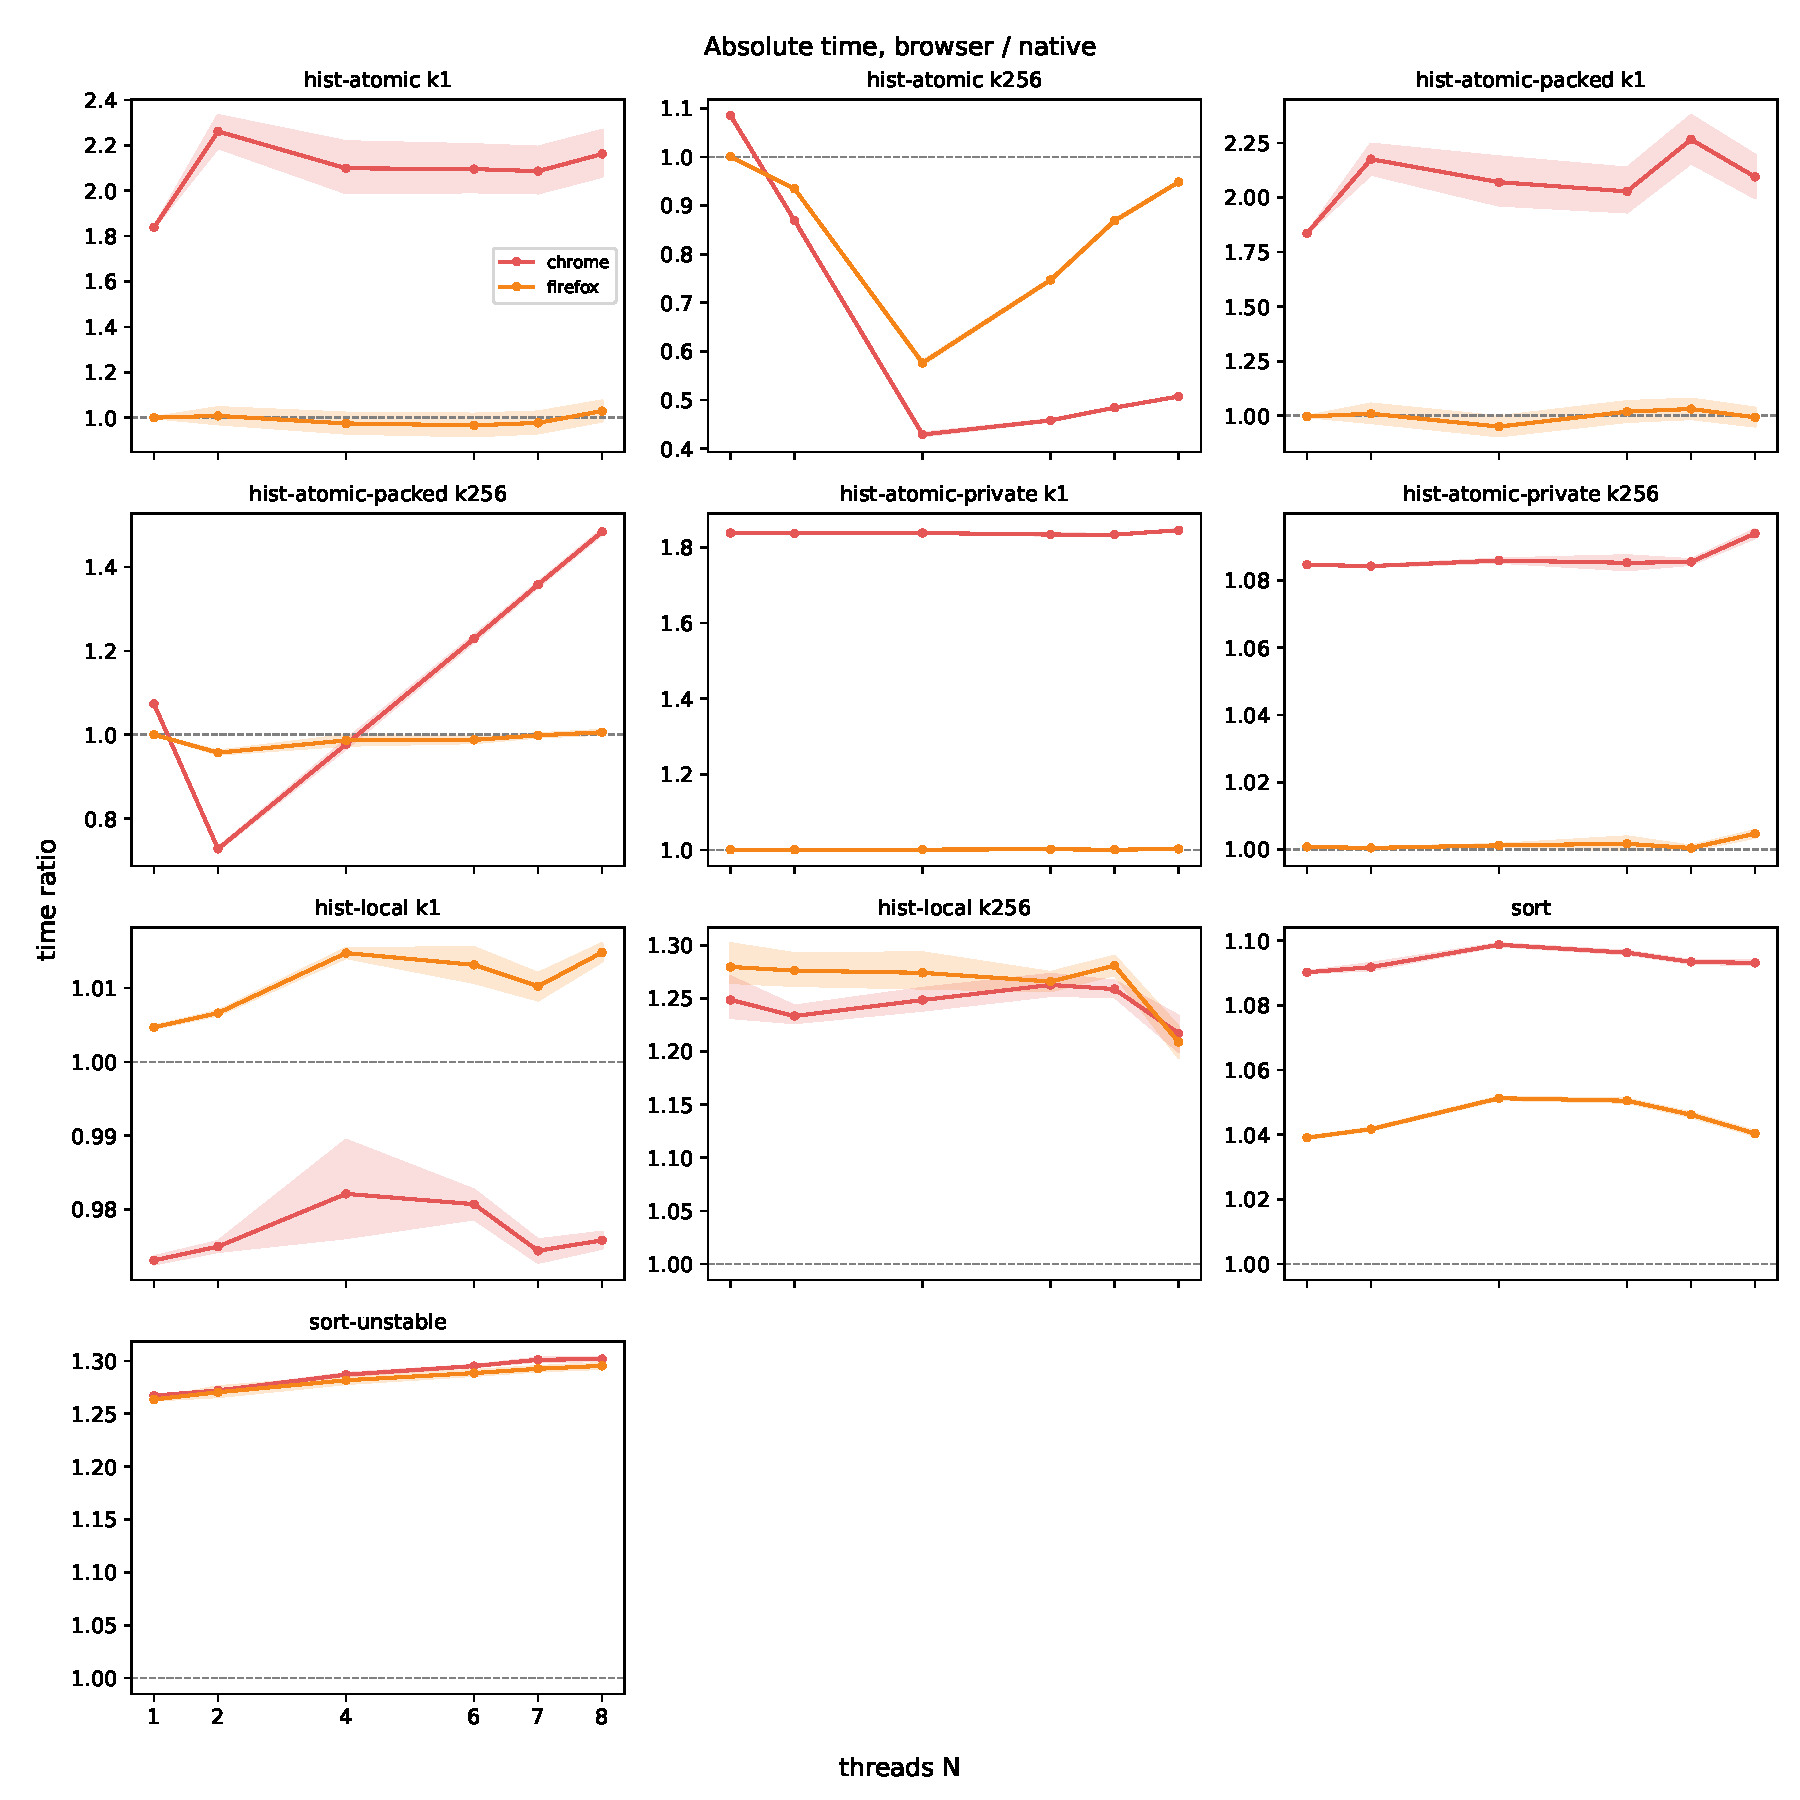
\includegraphics[width=0.8\linewidth]{../figures/extras-absolute.pdf}
\caption{Extras campaign: absolute time per workload and environment.}
\Description{Absolute time against thread count for the extras workloads.}
\label{fig:extras-absolute}
\end{figure}

\begin{figure}[tbp]
\centering
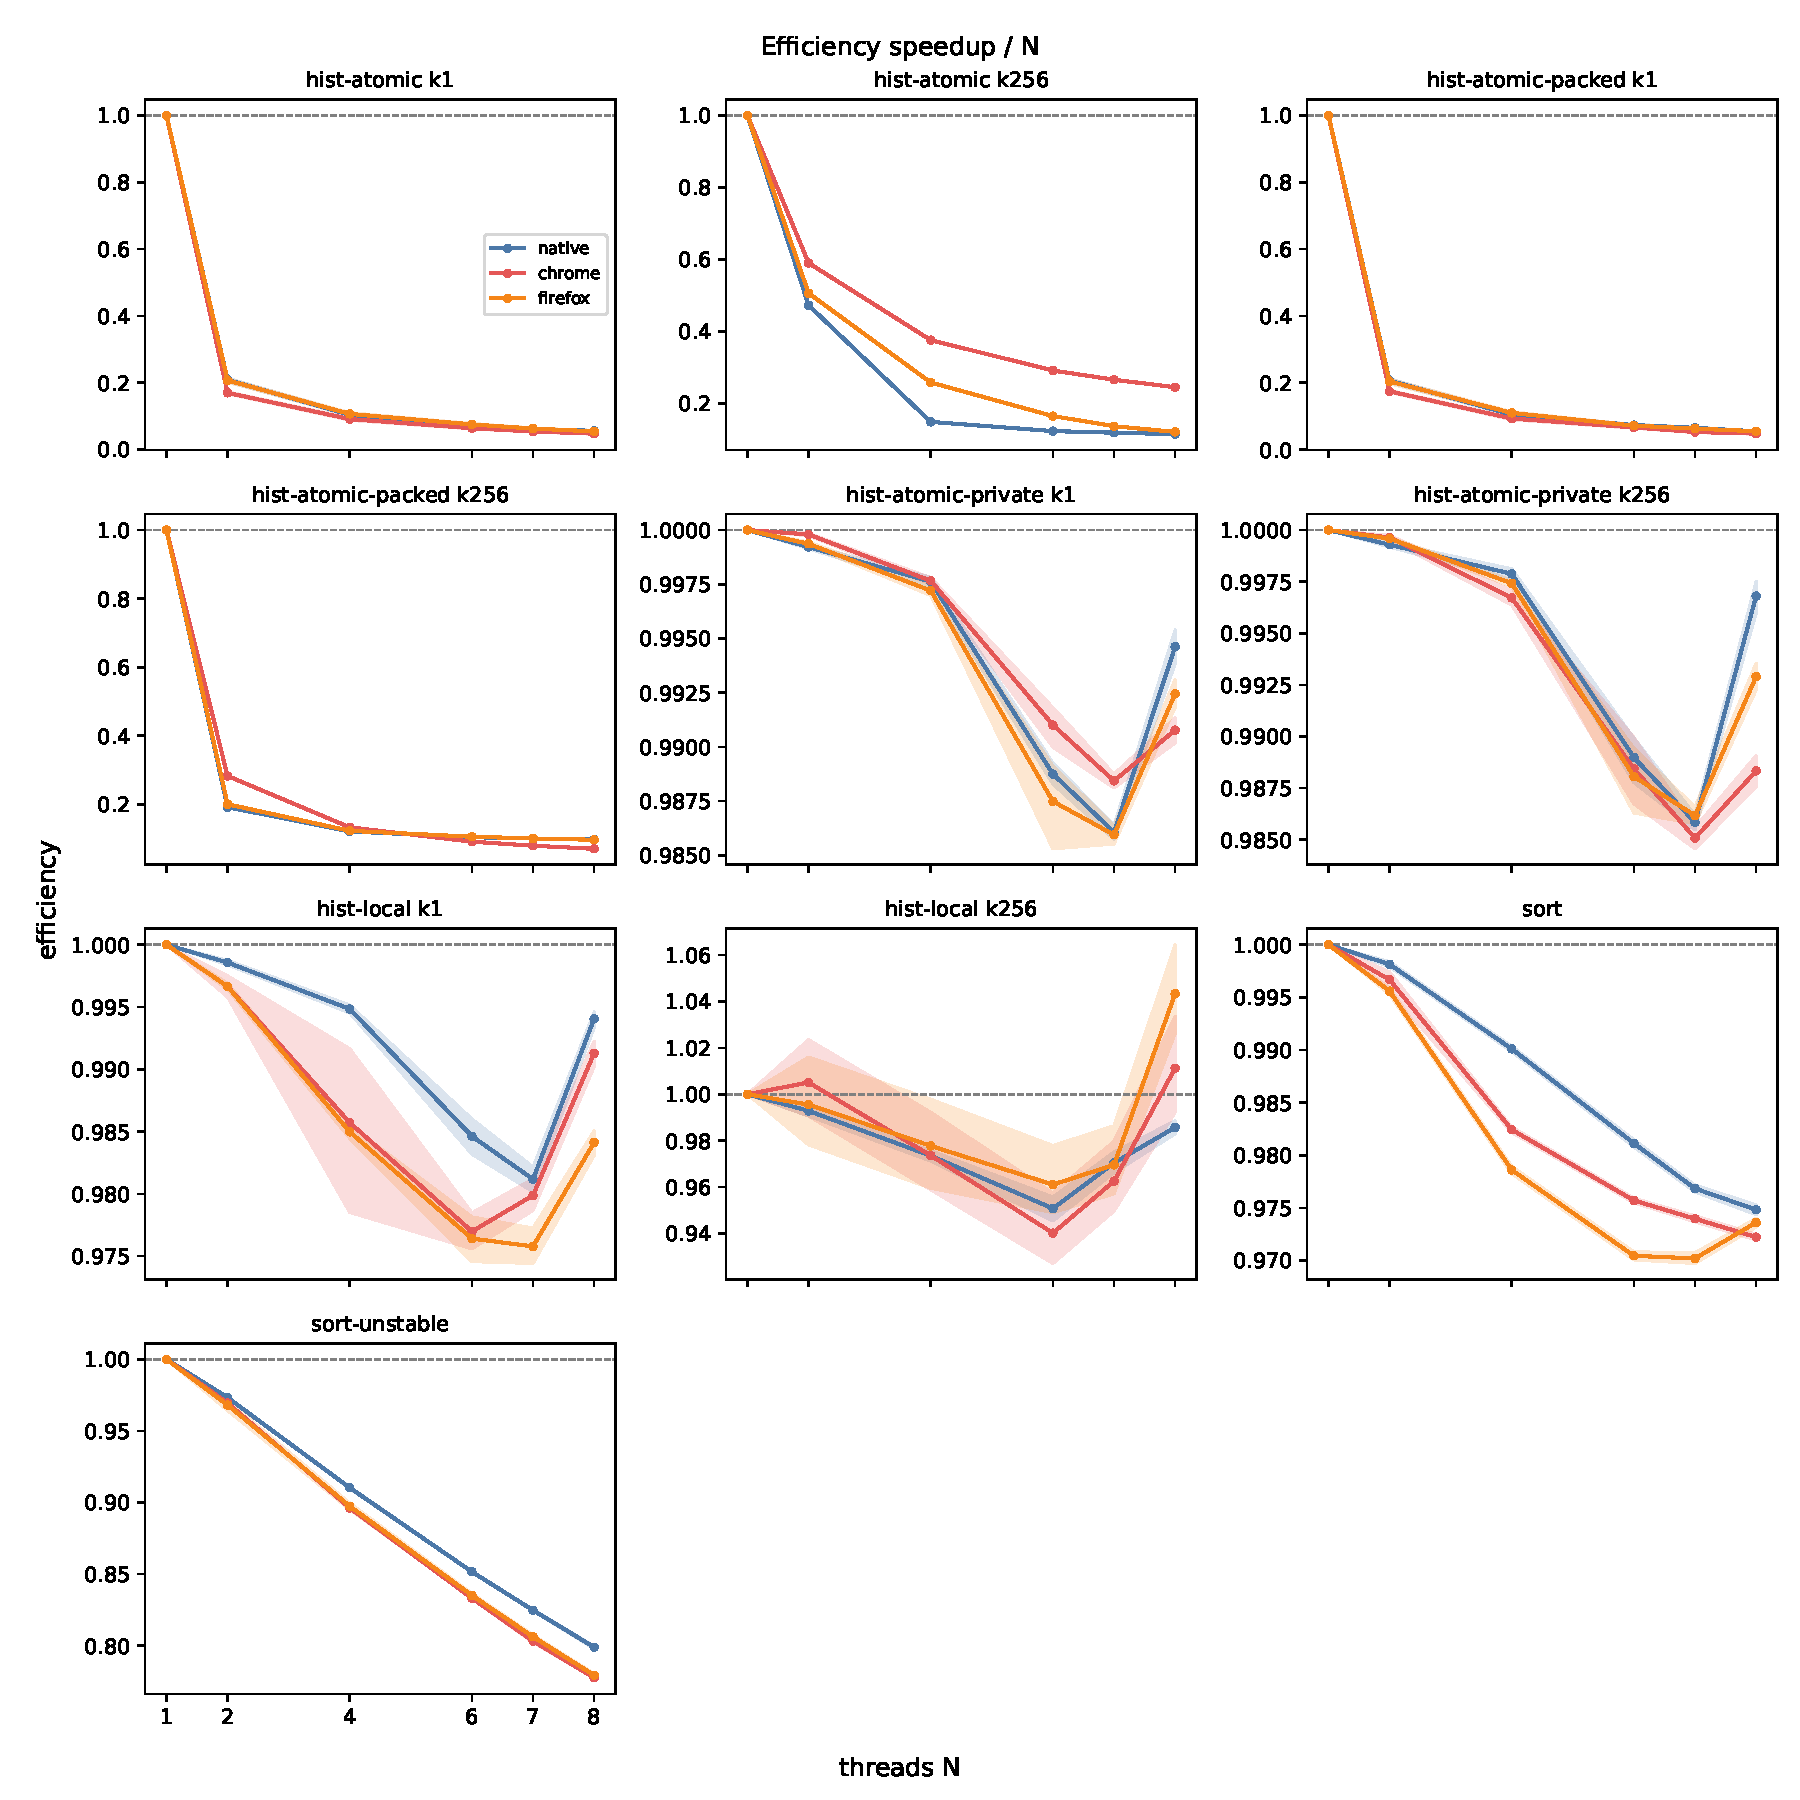
\includegraphics[width=0.8\linewidth]{../figures/extras-efficiency.pdf}
\caption{Extras campaign: efficiency per workload.}
\Description{Efficiency against thread count for the extras workloads.}
\label{fig:extras-efficiency}
\end{figure}

\begin{figure}[tbp]
\centering
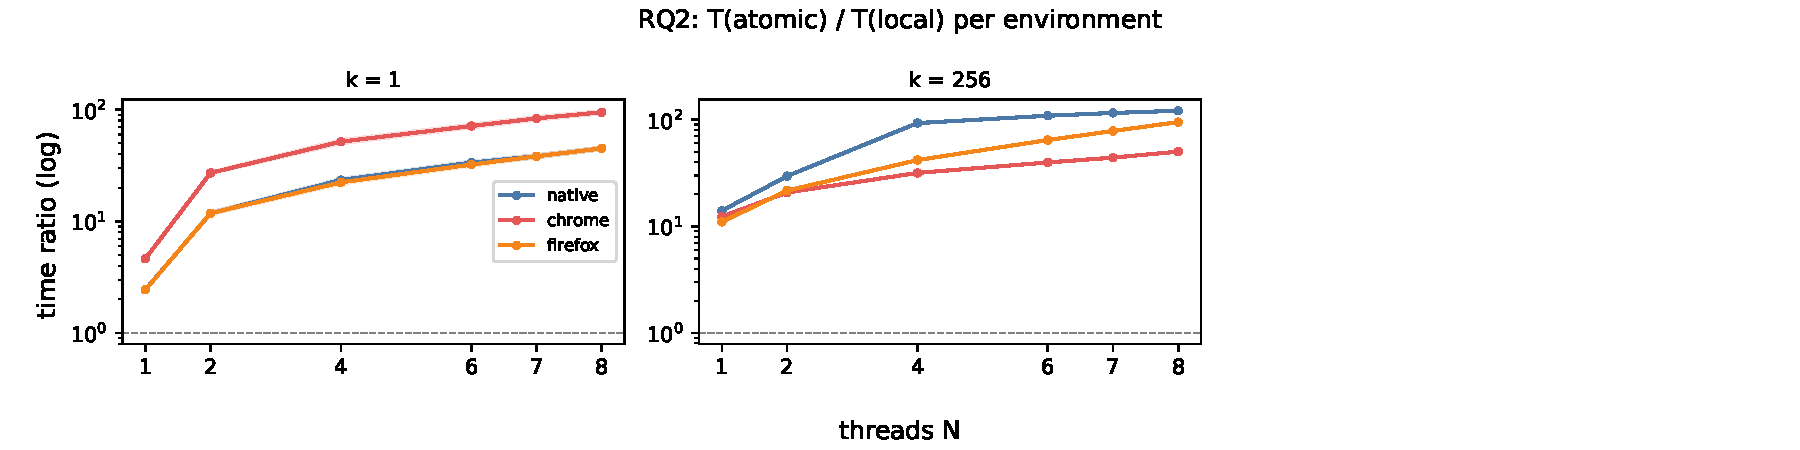
\includegraphics[width=\linewidth]{../figures/extras-rq2.pdf}
\caption{Extras campaign: $T_{\mathrm{atomic}}/T_{\mathrm{local}}$ against
$N$ for the shared padded atomics at $k=1$ and 256, measured again.}
\Description{Atomic over local time ratio against thread count in the extras campaign.}
\label{fig:extras-rq2}
\end{figure}

\begin{itemize}[leftmargin=1.5em]
\item \emph{The cells shared with the main campaign reproduce it.} The
local and shared histograms at $k=1$ and 256 were measured again,
interleaved, in this campaign: for example the shared atomics at $k=256$,
$N=8$ take 414.6, 210.3 and 392.8~ms here against 414.6, 210.4 and 393.0 in
the main campaign.
\item \emph{Private atomics scale like the local control} (speedup 7.90 to
7.96 in the three environments): the atomic instruction alone does not hurt
scaling. But it costs Chrome 88.0~ms at $k=1$, $N=8$ against 47.7~ms
natively and 47.8 in Firefox (1.85 times), and 52.1 against 47.7~ms at
$k=256$ (1.09 times). No line is shared here, so this is the cost of V8's
sequence without contention; it has the shape the native probe found for
the compare-and-swap with one thread (slower at $k=1$, close to the locked
add at $k=256$). Firefox matches native. Shared against private then gives
the part that contention adds: at $k=1$ Chrome's shared histogram takes
2.06 times the native one where its private one takes 1.85 times.
\item \emph{Packing the counters removes Chrome's advantage.} With eight
counters per line the atomic histogram at $k=256$, $N=8$ slows by 1.18
times natively (490 against 415~ms), 1.25 times in Firefox and 3.45 times
in Chrome (726 against 210~ms), which then takes 1.48 times the native
time. Chrome's advantage under spread contention depends on each counter
having its own line. At $k=1$ packing changes little (within 4\%): one counter is hit.
\item \emph{Sorts.} The stable parallel sort, which allocates, reaches
7.78 to 7.80 at $N=8$ in the three environments at 1.04 (Firefox) and 1.09
(Chrome) times the native time; the unstable in-place sort reaches 6.19 to
6.39 at 1.30 and 1.31 times. The sort that goes through WASM's allocator
does not show the larger gap, so the allocator's global lock is not visible
at this allocation rate.
\end{itemize}
One configuration trends with the execution order (Chrome, private, $k=1$,
$N=2$). Against the earlier build, every cell at eight threads is within
1\% of its v2 time except the two shared counters at $k=1$ (within 3.4\%),
the cells whose runs fall on levels; this is a consistency observation, not
a comparison of results.

\clearpage
\subsection{Weak scaling}

In strong scaling each thread gets $1/N$ of the work; in weak scaling the
input grows with $N$. The campaign (1080 runs) used an image 8192 pixels
wide and $1024N$ rows high, so that every thread gets the work it has in
the main campaign at $N=8$ (Table~\ref{tab:weak},
Figure~\ref{fig:weak}).

\begin{table}[htbp]
\caption{Weak scaling (1080 runs): the image is 8192 pixels wide and $1024N$ rows high. Time in ms and weak efficiency $T_1/T_N$ with its 95\,\% interval.}\label{tab:weak}
\centering\footnotesize
\begin{tabular}{llrcrcrc}
\toprule
 &  & \multicolumn{2}{c}{Native} & \multicolumn{2}{c}{Chrome} & \multicolumn{2}{c}{Firefox} \\
Workload & $N$ & $T_N$ & $T_1/T_N$ & $T_N$ & $T_1/T_N$ & $T_N$ & $T_1/T_N$ \\
\midrule
filter & 1 & 2.804 & 1.000 [1.000, 1.000] & 3.269 & 1.000 [1.000, 1.000] & 3.817 & 1.000 [1.000, 1.000] \\
filter & 2 & 3.007 & 0.932 [0.930, 0.935] & 3.492 & 0.936 [0.932, 0.941] & 4.011 & 0.951 [0.943, 0.960] \\
filter & 4 & 3.130 & 0.896 [0.893, 0.898] & 3.713 & 0.880 [0.875, 0.886] & 4.196 & 0.910 [0.902, 0.917] \\
filter & 6 & 3.164 & 0.886 [0.884, 0.888] & 3.807 & 0.859 [0.854, 0.863] & 4.222 & 0.904 [0.898, 0.910] \\
filter & 7 & 3.231 & 0.868 [0.866, 0.869] & 3.866 & 0.845 [0.841, 0.850] & 4.226 & 0.903 [0.898, 0.908] \\
filter & 8 & 3.259 & 0.860 [0.858, 0.863] & 3.843 & 0.851 [0.847, 0.855] & 4.172 & 0.915 [0.908, 0.922] \\
\midrule
local, $k$=1 & 1 & 19.427 & 1.000 [1.000, 1.000] & 18.867 & 1.000 [1.000, 1.000] & 19.672 & 1.000 [1.000, 1.000] \\
local, $k$=1 & 2 & 19.451 & 0.999 [0.998, 0.999] & 18.928 & 0.997 [0.995, 0.998] & 19.772 & 0.995 [0.994, 0.996] \\
local, $k$=1 & 4 & 19.519 & 0.995 [0.994, 0.996] & 18.996 & 0.993 [0.992, 0.994] & 19.803 & 0.993 [0.992, 0.994] \\
local, $k$=1 & 6 & 19.800 & 0.981 [0.979, 0.983] & 19.223 & 0.981 [0.978, 0.985] & 20.010 & 0.983 [0.981, 0.985] \\
local, $k$=1 & 7 & 19.718 & 0.985 [0.982, 0.988] & 19.216 & 0.982 [0.979, 0.985] & 19.947 & 0.986 [0.985, 0.988] \\
local, $k$=1 & 8 & 19.488 & 0.997 [0.996, 0.998] & 19.007 & 0.993 [0.992, 0.994] & 19.790 & 0.994 [0.993, 0.995] \\
\bottomrule
\end{tabular}
\end{table}


\begin{figure}[tbp]
\centering
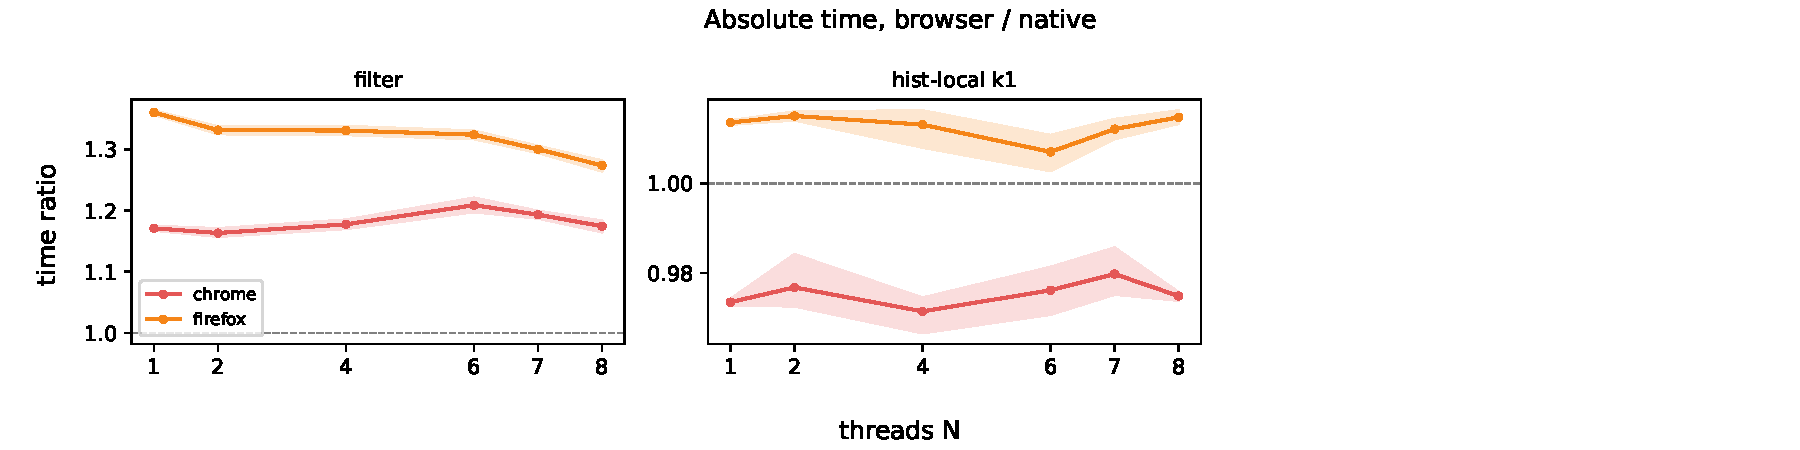
\includegraphics[width=0.75\linewidth]{../figures/weak-absolute.pdf}
\caption{Weak scaling: absolute time against $N$ (ideal: flat).}
\Description{Absolute time against thread count in weak scaling for the filter and the local histogram.}
\label{fig:weak}
\end{figure}

At eight threads the filter keeps 0.860 of its one-thread rate natively
[0.858, 0.863], 0.851 in Chrome and 0.915 in Firefox; the local histogram
0.993 to 0.997. These are the strong-scaling efficiencies (0.869, 0.865,
0.917) within one to two points: the filter's loss is the same whether the
work per thread shrinks or stays fixed, which fits a cost of sharing the
memory and not a serial part. The browser over native time ratio stays flat
in Chrome (1.16 to 1.20) and falls in Firefox from 1.36 at $N=1$ to 1.28 at
$N=8$.

\clearpage
\subsection{E-cores}

The hybrid campaign (900 runs) put the eight P-cores and twelve E-cores in
the mask and ran $N$ up to 20, to see how work stealing copes with cores of
two speeds (Table~\ref{tab:hybrid}, Figures~\ref{fig:hybrid-speedup}
and~\ref{fig:hybrid-absolute}).

\begin{table}[htbp]
\caption{Hybrid campaign (900 runs): 8 P-cores and 12 E-cores in the mask. Time in ms and speedup $T_1/T_N$ with its 95\,\% interval.}\label{tab:hybrid}
\centering\footnotesize
\begin{tabular}{llrcrcrc}
\toprule
 &  & \multicolumn{2}{c}{Native} & \multicolumn{2}{c}{Chrome} & \multicolumn{2}{c}{Firefox} \\
Workload & $N$ & $T_N$ & $S_N$ & $T_N$ & $S_N$ & $T_N$ & $S_N$ \\
\midrule
filter & 1 & 22.628 & 1.000 [1.000, 1.000] & 26.487 & 1.000 [1.000, 1.000] & 30.774 & 1.000 [1.000, 1.000] \\
filter & 8 & 3.503 & 6.460 [6.330, 6.569] & 4.046 & 6.547 [6.487, 6.601] & 4.385 & 7.018 [6.934, 7.096] \\
filter & 12 & 3.028 & 7.472 [7.303, 7.627] & 3.484 & 7.603 [7.544, 7.660] & 3.739 & 8.231 [8.135, 8.326] \\
filter & 16 & 2.879 & 7.861 [7.815, 7.904] & 3.463 & 7.648 [7.591, 7.706] & 3.551 & 8.666 [8.604, 8.726] \\
filter & 20 & 2.827 & 8.005 [7.978, 8.032] & 3.475 & 7.622 [7.584, 7.659] & 3.569 & 8.622 [8.556, 8.687] \\
\midrule
local, $k$=1 & 1 & 154.9 & 1.000 [1.000, 1.000] & 150.7 & 1.000 [1.000, 1.000] & 155.7 & 1.000 [1.000, 1.000] \\
local, $k$=1 & 8 & 19.631 & 7.893 [7.860, 7.935] & 18.655 & 8.078 [7.907, 8.280] & 19.830 & 7.850 [7.808, 7.907] \\
local, $k$=1 & 12 & 11.568 & 13.394 [13.209, 13.609] & 8.893 & 16.946 [16.578, 17.364] & 10.320 & 15.084 [14.805, 15.366] \\
local, $k$=1 & 16 & 7.973 & 19.433 [19.195, 19.683] & 5.979 & 25.207 [24.908, 25.509] & 7.432 & 20.945 [20.476, 21.421] \\
local, $k$=1 & 20 & 6.078 & 25.495 [25.046, 25.915] & 5.112 & 29.480 [28.850, 30.092] & 6.140 & 25.353 [25.039, 25.688] \\
\bottomrule
\end{tabular}
\end{table}


\begin{figure}[tbp]
\centering
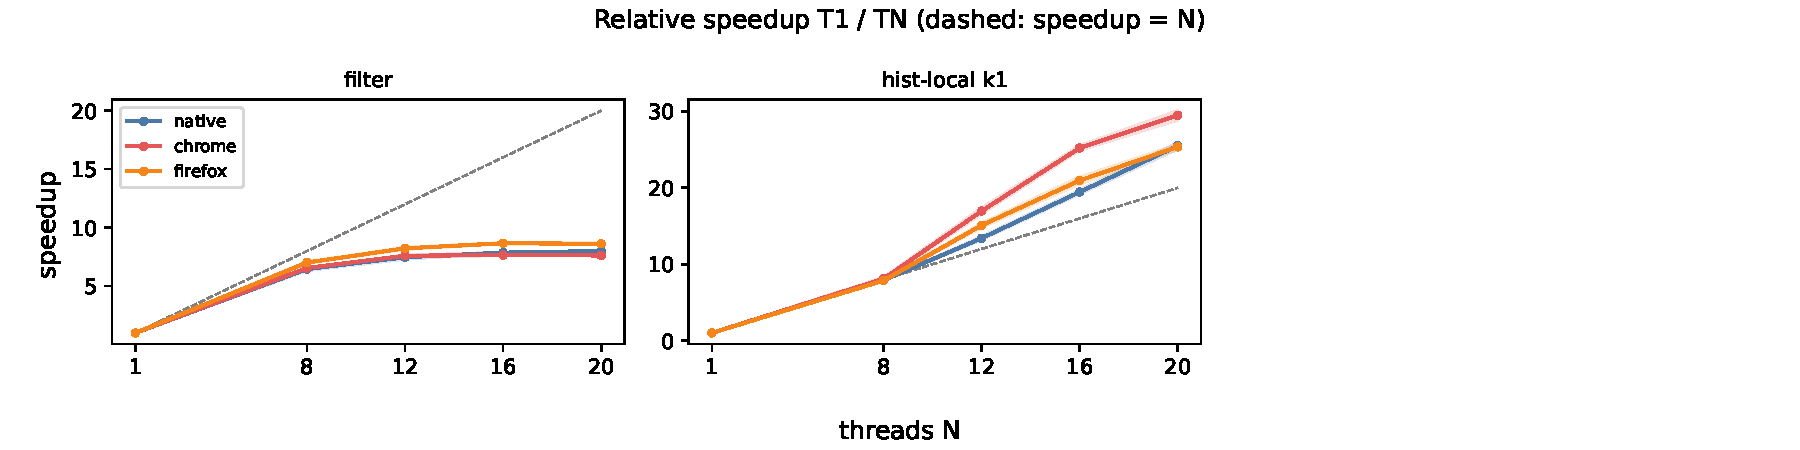
\includegraphics[width=0.75\linewidth]{../figures/hybrid-speedup.pdf}
\caption{Hybrid campaign: speedup against $N$ with P-cores and E-cores.}
\Description{Speedup against thread count up to twenty threads for the filter and the local histogram.}
\label{fig:hybrid-speedup}
\end{figure}

\begin{figure}[tbp]
\centering
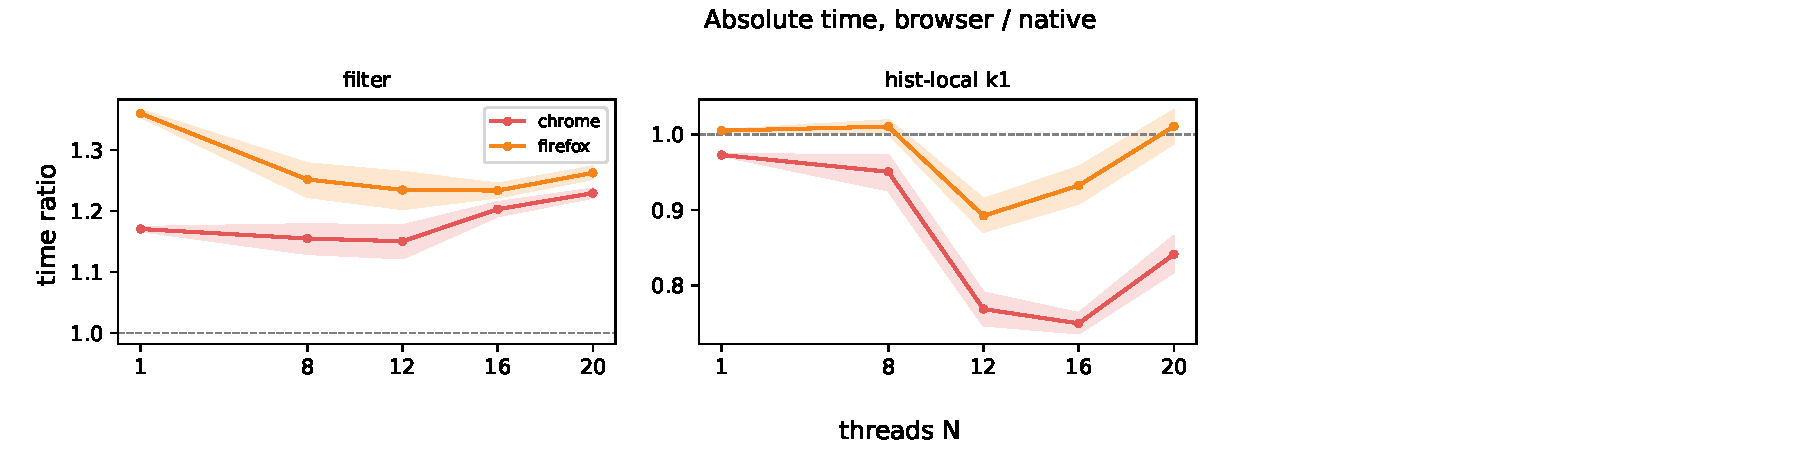
\includegraphics[width=0.75\linewidth]{../figures/hybrid-absolute.pdf}
\caption{Hybrid campaign: absolute time against $N$.}
\Description{Absolute time against thread count up to twenty threads.}
\label{fig:hybrid-absolute}
\end{figure}

The filter gains little from the E-cores: its speedup goes from 6.46 at
eight threads to 8.01 at twenty natively, 6.55 to 7.62 in Chrome and 7.02
to 8.62 in Firefox; in Chrome it is flat from twelve threads on. The three
environments use the extra cores about alike. The local histogram at $k=1$
goes far beyond the thread count (25.5 natively, 29.5 in Chrome and 25.4 in
Firefox at twenty threads): its one-thread time is a dependent chain on a
P-core, and the analysis of the earlier build traced the excess to the
E-cores running that chain faster than the P-cores do. Which threads the
kernel puts on which kind of core is not controlled and not recorded per
thread, and the cells with E-cores vary more than the others. With the
wider mask the eight-thread cells are slower than in the P-only campaign
(native filter 3.50 against 3.25~ms), as the mask pilot had found.

\clearpage
\subsection{Small regions: the cutoff}
\label{sec:cutoff}

RQ1 is answered at one size, where the work of a parallel region dominates
its fixed cost. The cutoff campaigns ask where that stops: five image sides
from 512 to 8192, $N \in \{1,2,4,8\}$, the filter and the local histogram
at $k=256$ (3600 runs, plus 480 native control runs). A 512$^2$ filter on
eight threads takes about 26~\textmu s natively, far under the 2~ms that
100 ticks of Firefox's clock need, so each timed sample repeats the work
$K = (8192/\mathrm{side})^2$ times and reports the time per pass. Sizes are
compared only through speedups within a size, where $K$ cancels
(Table~\ref{tab:cutoff}, Figure~\ref{fig:cutoff}).

\begin{figure}[tbp]
\centering
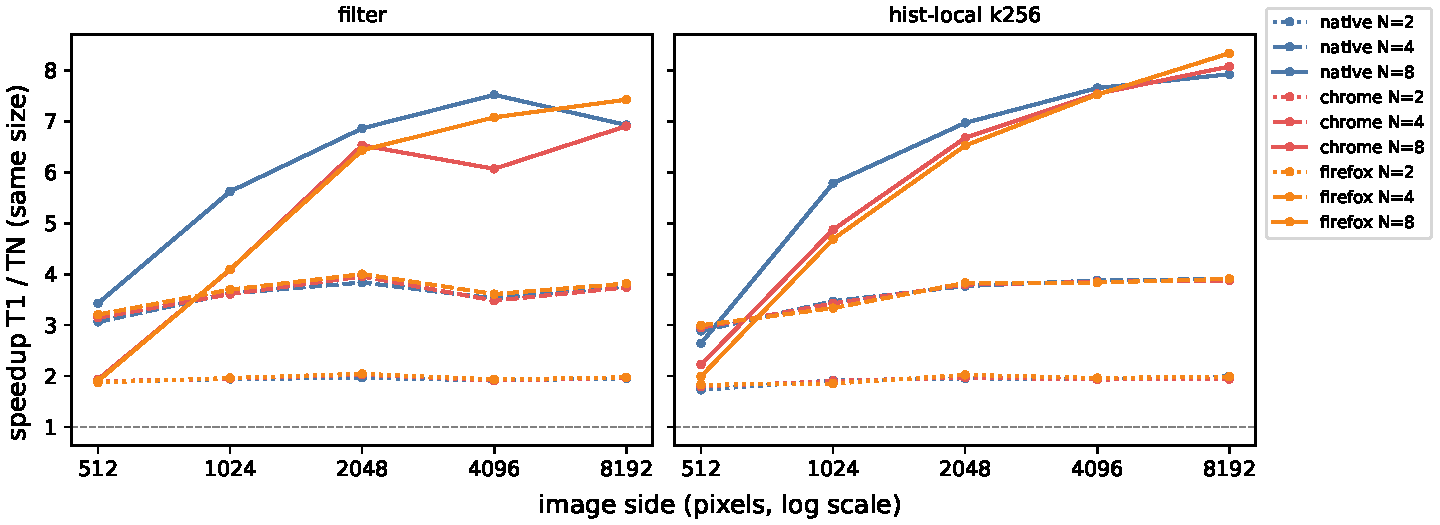
\includegraphics[width=\linewidth]{../figures/cutoff-speedup.pdf}
\caption{Cutoff campaigns: speedup against the image side, per environment
and $N$.}
\Description{Speedup against image side from 512 to 8192 for the filter and the local histogram in the three environments.}
\label{fig:cutoff}
\end{figure}

{\footnotesize
\begin{longtable}{lllccccc}
\caption{Cutoff campaigns: speedup (efficiency) by image side, with repeated passes per timed sample so that small images clear the clock.}\label{tab:cutoff} \\
\toprule
Workload & $N$ & Environment & 512$^2$ & 1024$^2$ & 2048$^2$ & 4096$^2$ & 8192$^2$ \\
\midrule
\endfirsthead
\toprule
Workload & $N$ & Environment & 512$^2$ & 1024$^2$ & 2048$^2$ & 4096$^2$ & 8192$^2$ \\
\midrule
\endhead
\bottomrule
\endfoot
filter & 2 & Native & 1.890 (0.945) & 1.944 (0.972) & 1.968 (0.984) & 1.913 (0.957) & 1.959 (0.979) \\
filter & 2 & Chrome & 1.900 (0.950) & 1.951 (0.975) & 2.029 (1.014) & 1.914 (0.957) & 1.970 (0.985) \\
filter & 2 & Firefox & 1.877 (0.939) & 1.964 (0.982) & 2.047 (1.023) & 1.935 (0.967) & 1.980 (0.990) \\
filter & 4 & Native & 3.063 (0.766) & 3.622 (0.906) & 3.837 (0.959) & 3.523 (0.881) & 3.775 (0.944) \\
filter & 4 & Chrome & 3.145 (0.786) & 3.610 (0.903) & 3.957 (0.989) & 3.481 (0.870) & 3.741 (0.935) \\
filter & 4 & Firefox & 3.207 (0.802) & 3.697 (0.924) & 4.001 (1.000) & 3.610 (0.902) & 3.817 (0.954) \\
filter & 8 & Native & 3.428 (0.429) & 5.622 (0.703) & 6.860 (0.857) & 7.519 (0.940) & 6.926 (0.866) \\
filter & 8 & Chrome & 1.936 (0.242) & 4.086 (0.511) & 6.528 (0.816) & 6.067 (0.758) & 6.905 (0.863) \\
filter & 8 & Firefox & 1.906 (0.238) & 4.095 (0.512) & 6.430 (0.804) & 7.077 (0.885) & 7.424 (0.928) \\
\midrule
local, $k$=256 & 2 & Native & 1.731 (0.866) & 1.918 (0.959) & 1.957 (0.979) & 1.940 (0.970) & 1.995 (0.998) \\
local, $k$=256 & 2 & Chrome & 1.798 (0.899) & 1.907 (0.953) & 1.974 (0.987) & 1.935 (0.967) & 1.943 (0.971) \\
local, $k$=256 & 2 & Firefox & 1.831 (0.916) & 1.855 (0.927) & 2.024 (1.012) & 1.964 (0.982) & 1.991 (0.996) \\
local, $k$=256 & 4 & Native & 2.887 (0.722) & 3.470 (0.868) & 3.768 (0.942) & 3.877 (0.969) & 3.906 (0.977) \\
local, $k$=256 & 4 & Chrome & 2.950 (0.738) & 3.428 (0.857) & 3.796 (0.949) & 3.850 (0.962) & 3.877 (0.969) \\
local, $k$=256 & 4 & Firefox & 2.998 (0.749) & 3.335 (0.834) & 3.830 (0.957) & 3.836 (0.959) & 3.909 (0.977) \\
local, $k$=256 & 8 & Native & 2.644 (0.330) & 5.786 (0.723) & 6.968 (0.871) & 7.651 (0.956) & 7.923 (0.990) \\
local, $k$=256 & 8 & Chrome & 2.227 (0.278) & 4.872 (0.609) & 6.674 (0.834) & 7.538 (0.942) & 8.074 (1.009) \\
local, $k$=256 & 8 & Firefox & 1.995 (0.249) & 4.688 (0.586) & 6.523 (0.815) & 7.523 (0.940) & 8.334 (1.042) \\
\end{longtable}
}

\begin{table}[htbp]
\caption{Cutoff at $N=8$: the image side at which the efficiency crosses 0.5 (interpolated, 95\,\% interval) and the sequential work of that image in \textmu s; then the fork-join model $T_N=W/N+F$ with this campaign's warm fork-join $F$ in \textmu s: the work it predicts for efficiency 0.5, and the side at which $F$ is 1\,\% and 5\,\% of $T_N$.}\label{tab:cutoff-estimates}
\centering\footnotesize
\begin{tabular}{llcrrrrr}
\toprule
Workload & Environment & Side at 0.5 & Work & $F$ & Model & Side 1\,\% & Side 5\,\% \\
\midrule
filter & Native & 613 [610, 616] & 124.9 & 10.8 & 86.1 & 5031 & 2204 \\
local, $k$=256 & Native & 691 [679, 701] & 183.4 & 10.8 & 86.1 & 4595 & 2013 \\
filter & Chrome & 996 [989, 1002] & 395.6 & 105.0 & 840.0 & 14518 & 6360 \\
local, $k$=256 & Chrome & 815 [797, 832] & 324.6 & 105.0 & 840.0 & 12938 & 5668 \\
filter & Firefox & 994 [976, 1009] & 459.4 & 60.0 & 480.0 & 10151 & 4447 \\
local, $k$=256 & Firefox & 858 [840, 873] & 361.9 & 60.0 & 480.0 & 9607 & 4209 \\
\bottomrule
\end{tabular}
\end{table}


\begin{figure}[tbp]
\centering
\begin{tikzpicture}[font=\scriptsize, x=1cm, y=1cm]
  \node[anchor=east] at (0,1.5) {large region};
  \draw[fill=native!20] (0.1,1.25) rectangle ++(6.0,0.5) node[midway] {work $W/N$};
  \draw[fill=chrome!30] (6.1,1.25) rectangle ++(0.25,0.5);
  \node[anchor=west] at (6.45,1.5) {$F$: under 3\% of $T_N$};
  \node[anchor=east] at (0,0.6) {small region};
  \draw[fill=native!20] (0.1,0.35) rectangle ++(0.9,0.5) node[midway] {$W/N$};
  \draw[fill=chrome!30] (1.0,0.35) rectangle ++(0.9,0.5) node[midway] {$F$};
  \node[anchor=west] at (2.0,0.6) {$W = NF$: half of $T_N$ is fork-join, efficiency 0.5};
\end{tikzpicture}
\caption{The fork-join model $T_N = W/N + F$. The work of a region divides
by $N$; its fixed cost $F$ does not, and $F$ is six to ten times larger in
the browsers.}
\Description{Two bars: a long bar of work with a small fork-join part, and a short bar where work and fork-join are equal.}
\label{fig:forkjoin-model}
\end{figure}

\begin{itemize}[leftmargin=1.5em]
\item \emph{No size measured reached break-even.} The speedup is above 1 at
every size and thread count, in every environment: even at 512$^2$ eight
threads give 3.4 natively and 1.9 in the browsers for the filter.
\item \emph{Worth it at half the ideal speedup.} At $N=8$ the efficiency
crosses 0.5 at a side of 613 natively and about 995 in both browsers for
the filter (Table~\ref{tab:cutoff-estimates}): 125~\textmu s of sequential
work natively, 396 in Chrome and 459 in Firefox. A region must hold about
three to four times more work in a browser than natively before eight
threads pay half of what they could.
\item \emph{The fork-join model} (Figure~\ref{fig:forkjoin-model}). $T_N = W/N + F$, with $W$ the work of a
region and $F$ the warm fork-join cost of these campaigns' calibration
(10.8, 105 and 60~\textmu s), predicts efficiency 0.5 at $W = NF$: 86, 840
and 480~\textmu s. The measured 125, 396 and 459 agree for Firefox, are 1.5
times the model natively and half of it in Chrome: the calibration's
broadcast is a barrier that every worker must run and overstates what an
ordinary region pays in Chrome. The model is a guide, not a fit.
\item \emph{The 100:1 rule.} A common rule asks that the fork overhead be
under 1\% of a region. At 8192$^2$ the warm fork-join is 0.33\% of $T_8$
natively, 1.4\% in Firefox and 2.7\% in Chrome; by that rule the browsers
would need images of about 10\,000$^2$ and 14\,500$^2$, larger than this
study measured.
\end{itemize}

\paragraph{The sizes are lower bounds for a single call.} With repeated
passes the workers are still awake between passes, which a single call does
not enjoy. Two native control campaigns ran one pass per sample: at 512$^2$
the filter on eight threads takes 33.0~\textmu s per call against
25.8~\textmu s per pass with 256 passes, and at 2048$^2$ 330 against
192~\textmu s, a speedup of 4.56 against 6.86 (the local histogram barely
changes there, 235 against 229~\textmu s). A program that calls a parallel
region once, cold, needs more work per region than the table says.

\clearpage
\subsection{Inside a region: the grain}
\label{sec:grain}

The other half of the question is the size of a task inside one region.
The grain sweeps (5400 runs at $N=8$) give every task a fixed size, in
powers of two, from one row or 1~KB up to one task per thread, with Rayon's
adaptive split as the reference (Table~\ref{tab:grain-best},
Figures~\ref{fig:grain} and~\ref{fig:grain-all}).

\begin{figure}[tbp]
\centering
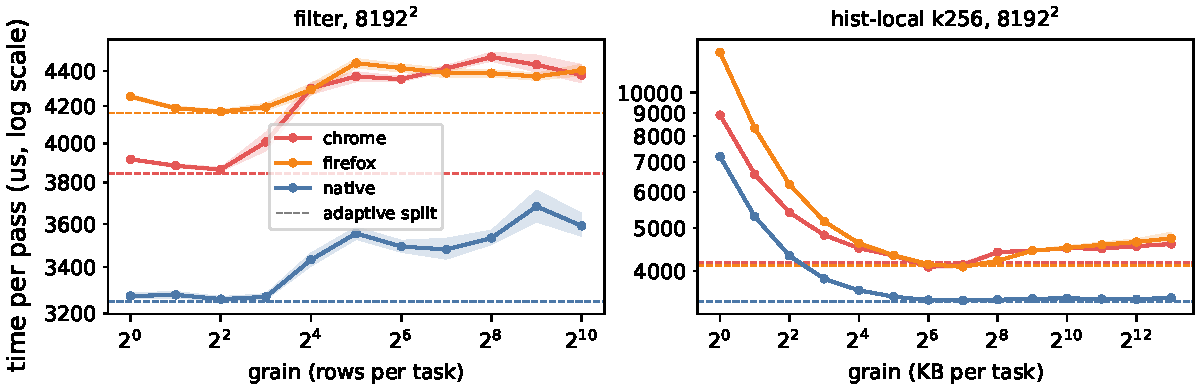
\includegraphics[width=0.8\linewidth]{../figures/grain-ucurve-8192.pdf}
\caption{Grain sweep at 8192$^2$, $N=8$: time per pass against the task
grain (log-log, 95\% CI); dashed: Rayon's adaptive split.}
\Description{Time per pass against task grain for the filter and the local histogram at 8192 squared, one line per environment.}
\label{fig:grain}
\end{figure}

\begin{figure}[tbp]
\centering
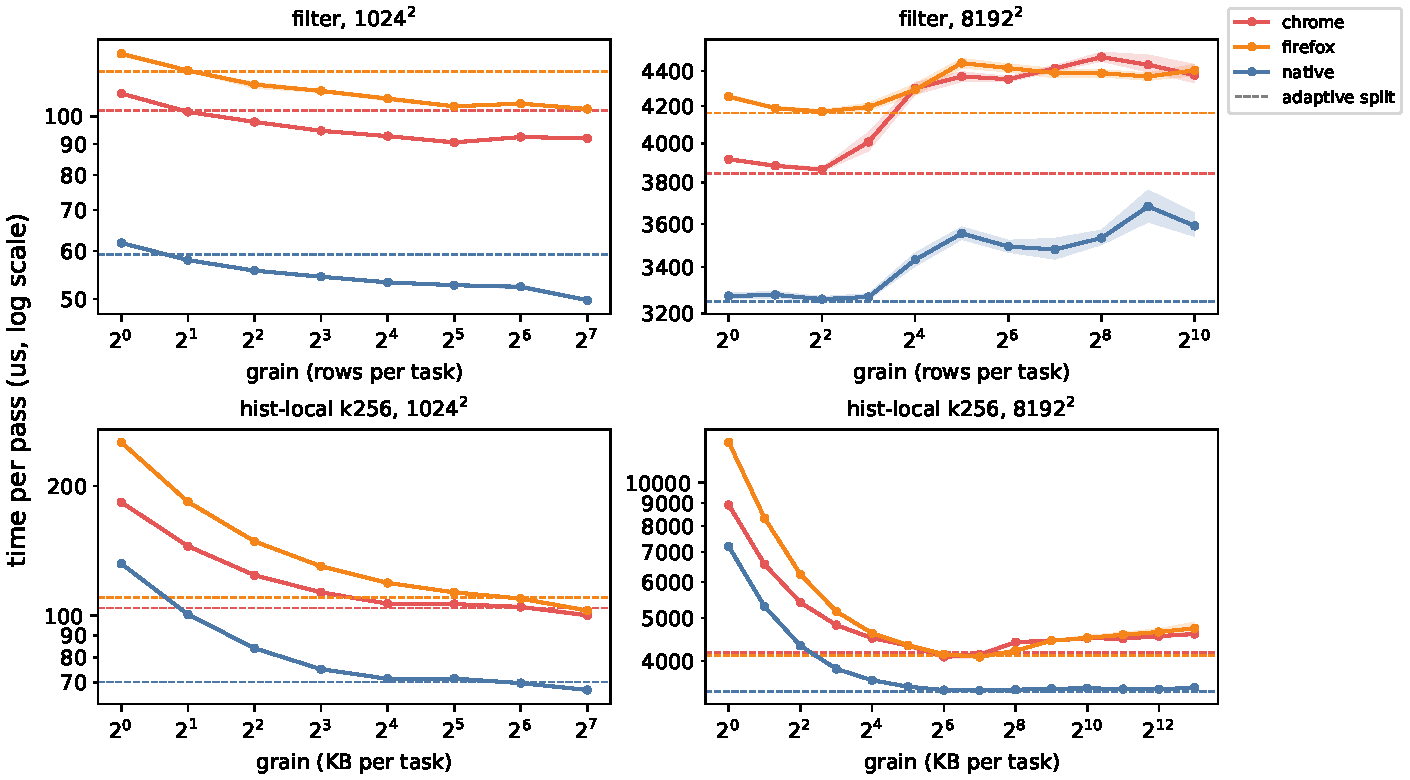
\includegraphics[width=\linewidth]{../figures/grain-ucurve.pdf}
\caption{Grain sweeps at both sizes and for every workload swept.}
\Description{Time per pass against task grain at 1024 squared and 8192 squared.}
\label{fig:grain-all}
\end{figure}

\begin{table}[htbp]
\caption{Grain sweeps at $N=8$: the best fixed grain (rows for the filter, KB for the histograms), its time per pass in \textmu s, the flat region (grains whose interval overlaps the best), Rayon's adaptive split over the best, and the cost of one task in ns with its 95\,\% interval.}\label{tab:grain-best}
\centering\footnotesize
\begin{tabular}{lllrrcrc}
\toprule
Side & Workload & Environment & Best & Time & Flat & Adaptive & Task cost \\
\midrule
1024$^2$ & filter & Chrome & 32 & 90.2 & 32 to 32 & 1.128 & 149 [143, 155] \\
1024$^2$ & filter & Firefox & 128 & 101.9 & 128 to 128 & 1.162 & 199 [191, 207] \\
1024$^2$ & filter & Native & 128 & 50.1 & 128 to 128 & 1.183 & 93 [89, 96] \\
1024$^2$ & local, $k$=256 & Chrome & 128 & 100.5 & 128 to 128 & 1.042 & 641 [631, 650] \\
1024$^2$ & local, $k$=256 & Firefox & 128 & 102.6 & 128 to 128 & 1.056 & 1197 [1189, 1205] \\
1024$^2$ & local, $k$=256 & Native & 128 & 67.5 & 128 to 128 & 1.029 & 504 [498, 510] \\
8192$^2$ & filter & Chrome & 4 & 3848.9 & 2 to 4 & 0.999 & 83 [48, 118] \\
8192$^2$ & filter & Firefox & 4 & 4190.8 & 2 to 8 & 0.996 & 85 [33, 137] \\
8192$^2$ & filter & Native & 4 & 3248.4 & 2 to 4 & 1.002 & 22 [6, 35] \\
8192$^2$ & atomic, $k$=256 & Chrome & 1 & 209470.4 & 1 to 8 & 1.004 & - \\
8192$^2$ & atomic, $k$=256 & Firefox & 4096 & 392514.2 & 512 to 8192 & 1.001 & 537 [481, 592] \\
8192$^2$ & atomic, $k$=256 & Native & 1 & 413763.2 & 1 to 128 & 1.002 & - \\
8192$^2$ & local, $k$=256 & Chrome & 64 & 4094.2 & 64 to 128 & 1.027 & 598 [589, 606] \\
8192$^2$ & local, $k$=256 & Firefox & 128 & 4071.2 & 64 to 128 & 1.010 & 1010 [1003, 1017] \\
8192$^2$ & local, $k$=256 & Native & 128 & 3434.5 & 128 to 256 & 0.995 & 461 [460, 462] \\
\bottomrule
\end{tabular}
\end{table}


\begin{itemize}[leftmargin=1.5em]
\item \emph{A U-curve, as expected.} For the local histogram at 8192$^2$,
tasks of 1~KB cost 2.1 times the best natively, 2.2 times in Chrome and 3.0
times in Firefox: each task builds and merges a 2~KB table. One task per
thread costs 1.01 times natively and 1.11 to 1.16 times in the browsers:
nothing is left to steal when a thread falls behind. For the filter the
curve is shallow: one row per task costs 0.5\% to 1.7\% more than the best,
and 1024 rows per task 7\% to 13\% more.
\item \emph{The best grain is the same in the three environments}: 4 rows
for the filter, 64 to 128~KB for the histogram. The browsers' fork-join is
six to ten times native's, yet their best grain is not coarser, because
what a task pays is not the region's fork-join but the cost of one task:
0.46~\textmu s natively, 0.60 in Chrome and 1.0 in Firefox for the
histogram. The 100:1 rule lands in the flat region when applied to that
cost (110, 117 and 201~KB).
\item \emph{Rayon's adaptive split is within 3\% of the best fixed grain at
8192$^2$} (0.995 to 1.027 times) and 3\% to 18\% slower at 1024$^2$. The
main campaign's use of the adaptive split costs it nothing at its size.
\item \emph{The atomic histogram hardly depends on the grain}: at $k=256$
its time over fifteen grains stays within 0.3\% of the best natively, 0.6\%
in Chrome and 1.3\% in Firefox. Its time is set by contention for the
counters. This also bounds what the v3 change to its task code could have
moved.
\end{itemize}
One feature is unexplained: between grains of 8 and 16 rows the filter
steps up by 4\% natively, 7\% in Chrome and 2\% in Firefox.
